\chapter{Testowanie systemu}

System został przetestowany manualnie poprzez interfejs graficzny oraz poprzez analizę zapytań SQL wykonywanych przez klasę \texttt{ZajeciaDAO}. Testy przeprowadzono w środowisku lokalnym z bazą danych \textbf{PostgreSQL}.

\section{Testy logowania}

Przetestowano poprawność działania formularza logowania.

\begin{figure}[H]
\centering
\begin{minipage}{0.45\textwidth}
\centering
\textbf{Poprawne logowanie – użytkownik uzyskuje dostęp do systemu}\\[0.5em]
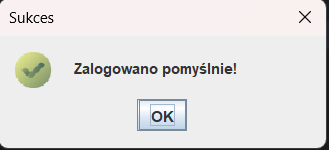
\includegraphics[width=\linewidth]{figures/approve/approve_login.png}
\caption{Logowanie zakończone sukcesem}
\label{fig:login-ok}
\end{minipage}
\hfill
\begin{minipage}{0.45\textwidth}
\centering
\textbf{Niepoprawne logowanie – system wyświetla komunikat błędu}\\[0.5em]
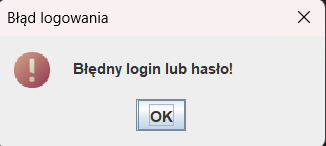
\includegraphics[width=\linewidth]{figures/Errors/bad_login.png}
\caption{Błąd logowania – nieprawidłowe dane}
\label{fig:login-fail}
\end{minipage}
\end{figure}

\section{Testy dodawania zajęć}

Przetestowano dodawanie różnych typów zajęć:

\begin{itemize}
    \item Dodanie zajęć typu \texttt{Projekt} – poprawne wstawienie danych do bazy;
    \item Sprawdzenie walidacji grupy i sali – przy próbie konfliktu system wyświetla stosowny komunikat;
    \item Dodanie zajęć tylko dla jednej grupy (np. \texttt{grupaA}) działa prawidłowo.
\end{itemize}

\begin{figure}[H]
\centering
\textbf{Pomyślne dodanie zajęć – system wyświetla komunikat potwierdzający}\\[0.5em]
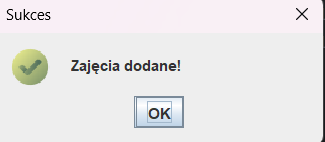
\includegraphics[width=0.5\textwidth]{figures/approve/add_zajecia_succesfull.png}
\caption{Potwierdzenie dodania zajęć}
\label{fig:added-success}
\end{figure}

\clearpage
\section{Testy filtrowania danych}

Sprawdzono poprawność działania filtrów:

\begin{itemize}
    \item Filtrowanie po dniu i grupie – poprawne ograniczenie wyników;
    \item Filtrowanie po typie zajęć i przedmiocie – wyświetlane są tylko pasujące rekordy;
    \item Filtrowanie nieistniejących danych – system poprawnie wyświetla pustą tabelę bez błędów.
\end{itemize}

\section{Testy edycji i usuwania zajęć}

Przetestowano operacje modyfikacji i usuwania danych:

\begin{itemize}
    \item Edycja sali i prowadzącego – zmiany są natychmiast widoczne w tabeli GUI;
    \item Usunięcie zajęć z bazy powoduje ich zniknięcie z interfejsu;
    \item Obsługa wyjątków SQL przy próbie edycji nieistniejącego rekordu działa prawidłowo.
\end{itemize}

\begin{figure}[H]
\centering
\textbf{Brak zaznaczonego wiersza – system przypomina o konieczności wyboru przed edycją}\\[0.5em]
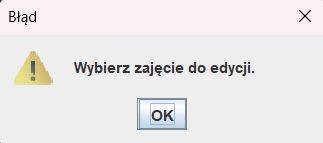
\includegraphics[width=0.5\textwidth]{figures/Warning/select_zajecia_to_edit.png}
\caption{Brak zaznaczonego rekordu do edycji}
\label{fig:warn-edit}
\end{figure}

\begin{figure}[H]
\centering
\textbf{Podczas usuwania rekordów użytkownik otrzymuje pytanie potwierdzające}\\[0.5em]
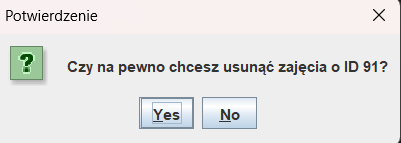
\includegraphics[width=0.5\textwidth]{figures/Warning/delete_warning.png}
\caption{Potwierdzenie usunięcia zajęć}
\label{fig:warn-delete}
\end{figure}

\begin{figure}[H]
\centering
\textbf{Brak zaznaczonego wiersza – system informuje o konieczności wyboru przed usunięciem}\\[0.5em]
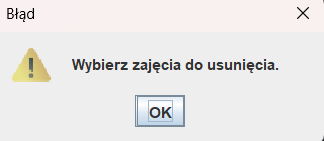
\includegraphics[width=0.5\textwidth]{figures/Warning/select_zajecia.png}
\caption{Brak zaznaczonego rekordu do usunięcia}
\label{fig:warn-no-selection}
\end{figure}

\section{Testy walidacji danych}

Sprawdzono poprawność działania walidacji formularza:

\begin{itemize}
    \item Puste pola – system wyświetla komunikat błędu i nie zapisuje danych;
    \item Nieprawidłowe dane (np. litery w polu godzina) – poprawna obsługa błędu i komunikat;
    \item Próba dodania zajęć do już zajętej sali – system blokuje takie dodanie;
    \item Konflikt grupy – użytkownik otrzymuje odpowiedni alert.
\end{itemize}

\begin{figure}[H]
\centering
\textbf{Użytkownik nie uzupełnił pól tekstowych — system wyświetla komunikat}\\[0.5em]
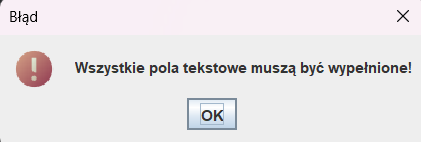
\includegraphics[width=0.55\textwidth]{figures/Errors/add_panel_error.png}
\caption{Puste pola formularza – komunikat błędu}
\label{fig:empty-fields}
\end{figure}

\textbf{Opis:} Ten fragment kodu sprawdza, czy pola formularza nie są puste. Jeśli są – zostaje wyświetlony komunikat, a operacja zostaje przerwana.

\begin{lstlisting}[caption={Walidacja pustych pól}, label={lst:puste}]
if (kierunek.isEmpty() || przedmiot.isEmpty() || prowadzacy.isEmpty()) {
    JOptionPane.showMessageDialog(null, "Wszystkie pola tekstowe musza byc wypelnione!",
        "Blad", JOptionPane.WARNING_MESSAGE, warningIcon);
    return;
}
\end{lstlisting}

\begin{figure}[H]
\centering
\textbf{Próba dodania zajęć do już zajętej sali — pojawia się komunikat o konflikcie}\\[0.5em]
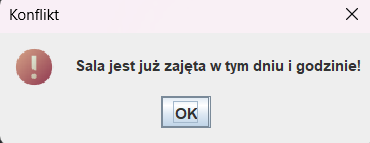
\includegraphics[width=0.55\textwidth]{figures/Errors/sala_zajeta_error.png}
\caption{Błąd – sala już zajęta w tym terminie}
\label{fig:room-taken}
\end{figure}

\textbf{Opis:} Fragment ten sprawdza, czy sala jest dostępna o wybranej porze. W razie konfliktu, informuje użytkownika i przerywa operację.

\begin{lstlisting}[caption={Sprawdzanie dostępności sali}, label={lst:sala}]
if (dao.czySalaZajeta(sala, dzien, godzina, null)) {
    JOptionPane.showMessageDialog(null, "Sala jest juz zajeta w tym dniu i godzinie!",
        "Konflikt", JOptionPane.WARNING_MESSAGE, warningIcon);
    return;
}
\end{lstlisting}

\textbf{Opis:} Ten kod odpowiada za informowanie użytkownika o konflikcie w harmonogramie danej grupy. Obsługuje przypadek, gdy grupa ma już zajęcia w wybranym terminie.

\begin{lstlisting}[caption={Sprawdzenie konfliktu grupy}, label={lst:grupa}]
JOptionPane.showMessageDialog(null, "Wybrana grupa ma juz zajecia w tym dniu i godzinie!",
    "Konflikt", JOptionPane.WARNING_MESSAGE, warningIcon);
return;
\end{lstlisting}
